\documentclass[a4paper, 10pt]{article}
\usepackage[margin=0.5in]{geometry}

\usepackage{blindtext}
\usepackage{multicol}
\usepackage{booktabs}
\usepackage{amsmath}
\usepackage{mathtools}
\usepackage{float}
\usepackage{graphicx}
\usepackage{enumitem}
\usepackage{hyperref}
\usepackage{comment}

\graphicspath{ {../outputs/}{../data/} }


\setlength{\columnsep}{1cm}
\title{ENPM 673: Perception for Autonomous Robots - Project 2}
\author{Aswath Muthuselvam \\ aswath@umd.edu}
\date{9th March 2022}

\begin{document}
\maketitle
\newlist{contract}{enumerate}{10}
\setlist[contract]{label*=\arabic*.}
\setlistdepth{10} 

\begin{figure}[b]
	\centering
	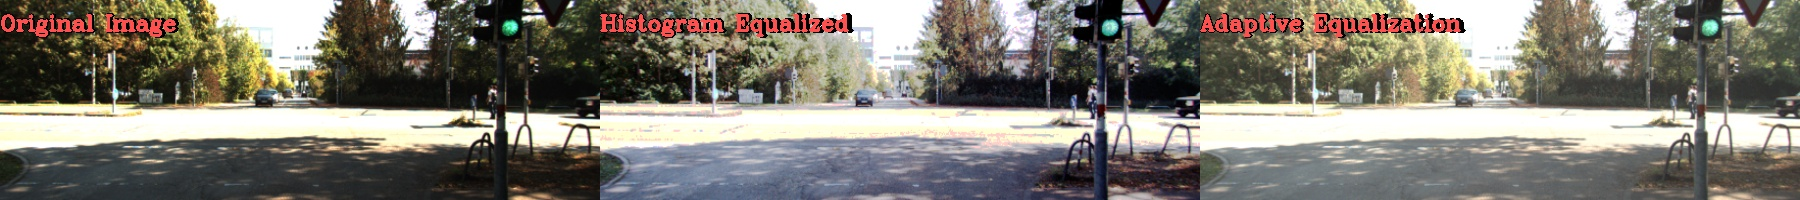
\includegraphics[width=\textwidth]{/histogram_and_adaptive.jpg}
	\caption{Original Image(left), Histogram Equalization(middle) and Adaptive Equalization(right)}
	\label{fig:HistEQ}
\end{figure}

\begin{multicols}{2}

\section{Histogram equalization}
The 24 images that was provided is taken and histogram is calculated with 256 bins, in all 3 channels-red, green and blue. Next, the cumulative distribution is calculated by summing all this bins till the current bin. This distribution is normalized and with a maximum  value of 256. A copy of this normalized value is also saved, this reduces the computation time as it can directly be applied to the subsequent $N$ video as they will have similar color distribution. The Adaptive equalization perform Gamma correction on the given image. The gamma correction of input pixel to output image is shown in Equation \ref{eq:gamma}. I took $\gamma$ is taken as 2.0.  The comparison between Original image, Histogram Equalized image and Adaptive Equalized image is shown in Figure \ref{fig:HistEQ} in the same order.

\begin{equation} \label{eq:gamma}
I_{out}=I_{in}^{\gamma}
\end{equation}
	
\section{Straight Lane Detection}

\blindtext
\section{Predict Turn}	

\end{multicols}


	
\end{document}
